\documentclass[11pt]{article}

% -----------------------------
% Packages
% -----------------------------
\usepackage[a4paper,margin=1in]{geometry}
\usepackage{microtype}
\usepackage{amsmath,amssymb,bm}
\usepackage{mathtools}
\usepackage{booktabs}
\usepackage{hyperref}
\usepackage{cleveref}
\usepackage{graphicx}
\usepackage{enumitem}
\usepackage{algorithm}
\usepackage{algpseudocode}
\usepackage{listings}
\usepackage{xcolor}
\usepackage{tikz}
\usepackage{float}
\usepackage[colorinlistoftodos]{todonotes}
\usetikzlibrary{arrows.meta,positioning,shapes.geometric}

% -----------------------------
% Hyperref
% -----------------------------
\hypersetup{
  colorlinks=true,
  linkcolor=blue,
  urlcolor=blue,
  citecolor=blue
}

% -----------------------------
% Listings (Julia)
% -----------------------------
\definecolor{codebg}{RGB}{248,248,248}
\definecolor{codekw}{RGB}{0,92,173}
\definecolor{codecm}{RGB}{90,90,90}
\definecolor{codestr}{RGB}{163,21,21}

\lstdefinelanguage{Julia}{
  morekeywords={mutable,struct,function,end,return,import,Base,for,if,else,elseif,while,break,continue,in,nothing,true,false},
  sensitive=true,
  morecomment=[l]{\#},
  morestring=[b]"
}

\lstset{
  language=Julia,
  basicstyle=\ttfamily\small,
  backgroundcolor=\color{codebg},
  frame=single,
  rulecolor=\color{black!15},
  frameround=tttt,
  tabsize=2,
  showstringspaces=false,
  breaklines=true,
  breakatwhitespace=true,
  keywordstyle=\color{codekw}\bfseries,
  commentstyle=\color{codecm}\itshape,
  stringstyle=\color{codestr},
  numbers=left,
  numberstyle=\tiny\color{black!45},
  numbersep=8pt,
  xleftmargin=2.2em,
  framexleftmargin=1.8em
}

\lstset{
  extendedchars=true,
  literate={∉}{{$\notin$}}1 {∈}{{$\in$}}1 {α}{{$\alpha$}}1 {δ}{{$\delta$}}1 {η}{{$\eta$}}1 {θ}{{$\theta$}}1 {λ}{{$\lambda$}}1 {μ}{{$\mu$}}1 {π}{{$\pi$}}1 {ρ}{{$\rho$}}1 {σ}{{$\sigma$}}1 {τ}{{$\tau$}}1 {ω}{{$\omega$}}1
}
% -----------------------------
% Title
% -----------------------------
\begin{document}
\begin{titlepage}
    \centering
    \includegraphics[width=0.7\textwidth]{NUS.png}
    \vspace*{0.2cm}
    
    {\huge \textbf{From Scratch: Reverse-Mode Automatic Differentiation and Integrated Gradients for Interpretability in Neural and Physics-Based Models} \par}
    
    \vspace{1.0cm}
    
    {\large \textbf{Course code: EE5311 Differentiable and Probabilistic Computing} \par}
    {\large Electrical and Computer Engineering \par}
    
    \vspace{1.0cm}
    
    {\large \textbf{Supervised By:} Prof. CHITRE, Mandar Anil \par}
    
    \vspace{1.0cm}
    
    {\large \textbf{Written By:} \par}
    {\large Liu Fei (A0275104M) \par}
    {\large Cao Yuan (A0275177U) \par}
    {\large Jin Xuan (A0328457U) \par}
    {\large Gao Jiaxuan (A0332428H) \par}
    {\large Nan Jinyao (A0319482X) \par}
    
    \vspace{0.8cm}
    
    {\large Date Last Edited: Feb 16, 2025 \par}
    
    \vfill
    
    \noindent\rule{\textwidth}{0.4pt}
    \vspace{0.1cm}
    \textbf{Declaration:} We understand what plagiarism is and have ensured We, Group 6, did not plagiarise for this assignment. We declare that our submission for CA1 Synthesis Essay is our own work. This assignment is in partial fulfilment of the requirements for the module EE5311.
    
    \vspace{0.2cm}
    \textbf{Declaration of AI-generated material:} During the preparation of this work, the author used generative AI tools (Google Gemini) to assist in LaTeX code generation (specifically for TikZ diagrams) and linguistic polishing. The author has reviewed and edited the content as needed and takes full responsibility for the content of the publication.
    \noindent\rule{\textwidth}{0.4pt}
\end{titlepage}

\begin{abstract}
We present a lightweight reverse-mode automatic differentiation (AD) engine implemented from scratch in Julia. The system builds dynamic computational graphs using a \texttt{Tensor} abstraction with operator overloading, and computes gradients via closure-based pullbacks (VJPs) scheduled by an iterative DFS topological traversal. Elementwise operations are supported through a broadcast-aware rule registry with shape-correct gradient reduction (\texttt{unbroadcast}). On top of this AD core, we implement Integrated Gradients (IG) for interpretability, supporting both AD-based gradients and finite differences for scalar black-box functions. Case studies on projectile-motion optimization and Iris MLP attribution demonstrate a unified pipeline for sensitivity analysis across physics-based and neural models. Our source code is available at: \url{https://github.com/nanjinyao/5311_CA1}.
\end{abstract}
``




\section{Introduction}

Automatic Differentiation (AD) is a foundational tool in modern scientific computing, enabling efficient and exact gradient computation for optimization, learning, and sensitivity analysis. While industrial frameworks provide highly optimized AD systems, understanding their internal mechanics is essential for both research transparency and algorithmic innovation. In this work, we implement a reverse-mode AD engine from scratch in Julia, emphasizing clarity, extensibility, and architectural rigor.

The system is built around a mutable \texttt{Tensor} abstraction that dynamically constructs computational graphs through operator overloading. Reverse-mode differentiation is implemented using closure-based Vector-Jacobian Products (VJPs) and executed via an iterative Depth-First Search (DFS) topological traversal, avoiding recursion limits and ensuring stable gradient scheduling.

A distinguishing feature of our implementation is a broadcast-aware differentiation mechanism. Instead of hard-coding elementwise operations, we integrate with Julia's broadcasting system through a custom \texttt{BroadcastStyle}. Backward rules for primitive functions (e.g., addition, multiplication, trigonometric and exponential functions) are managed via an extensible registry. To correctly propagate gradients through broadcasted operations, we introduce an \texttt{unbroadcast} operator that reduces gradients to their original operand shapes. This design separates forward semantics from backward logic and enables modular extension of differentiable primitives.

On top of the AD core, we implement Integrated Gradients (IG) as a unified attribution method for interpretability. The framework supports both AD-based gradients and finite-difference gradients for scalar-valued black-box functions, allowing consistent interpretability analysis across neural networks and differentiable physical models.

Through experiments on projectile-motion optimization and Iris classification, we demonstrate that gradients serve as a universal computational primitive bridging physics-based reasoning and deep learning interpretability.


\section{Core Principle: Chain Rule and Vector--Jacobian Products (VJP)}

Reverse-mode AD computes gradients efficiently for a scalar objective by repeatedly applying the chain rule along a computational graph. Let $L$ be a scalar output and let an intermediate node $u$ feed into one or more downstream nodes $v_1,\dots,v_k$. By the multivariate chain rule, the total derivative with respect to $u$ is the sum of all downstream contributions:
\begin{equation}
\frac{\partial L}{\partial u}
= \sum_{i=1}^{k} \frac{\partial L}{\partial v_i}\frac{\partial v_i}{\partial u}.
\label{eq:chain_rule_fanout}
\end{equation}
This ``fan-out'' case is ubiquitous in computational graphs: a value may be reused by multiple operators, so its gradient must accumulate contributions from multiple paths.

Our implementation follows the standard VJP (pullback) formulation used in reverse-mode AD. For each primitive operation producing $v = f(u)$, we do not form Jacobians explicitly. Instead, we store a local \emph{pullback} that maps the downstream sensitivity $g_v \triangleq \partial L/\partial v$ to the upstream sensitivity $g_u \triangleq \partial L/\partial u$:
\begin{equation}
g_u \; \mathrel{+}= \; g_v \cdot \frac{\partial f(u)}{\partial u},
\label{eq:vjp_update}
\end{equation}
where $\mathrel{+}=$ denotes in-place accumulation. In code, this corresponds to updating \texttt{parent.grad .+= ...} inside each node's \texttt{\_backward} closure. The closure captures any forward-pass context required to evaluate the local derivative (e.g., operands for multiplication, masks for ReLU, or cached broadcast results for certain elementwise functions).

By repeatedly executing these pullbacks in a valid reverse-topological order (from outputs back to inputs), the engine ensures that when a node's pullback is invoked, its \texttt{grad} field already contains the total accumulated $\partial L/\partial(\texttt{node})$ from all of its downstream consumers. This invariant enables correct gradient propagation without materializing large Jacobian matrices and forms the mathematical backbone of the reverse replay procedure used throughout the project.


\section{Core Abstraction: The \texttt{Tensor} Struct}

The entire AD engine is built around a mutable \texttt{Tensor} abstraction. Each \texttt{Tensor} instance represents a node in a dynamic computational graph and encapsulates both numerical data and the information required for reverse-mode differentiation.

\begin{lstlisting}[language=Julia, caption={Core Tensor abstraction from MiniAD.jl}]
mutable struct Tensor
    data::Array{Float64}
    grad::Array{Float64}
    _backward::Function
    _prev::Set{Tensor}
    op::String
    requires_grad::Bool

    function Tensor(data; _children=(), _op="", requires_grad=true)
        d = if data isa Number
            reshape([Float64(data)], 1, 1)
        else
            arr = convert(Array{Float64}, data)
            ndims(arr) == 1 ? reshape(arr, :, 1) : arr
        end

        g = zeros(size(d))
        prev = requires_grad ? Set{Tensor}(_children) : Set{Tensor}()
        new(d, g, () -> nothing, prev, _op, requires_grad)
    end
end
\end{lstlisting}

\subsection{Design Principles}

\paragraph{Uniform 2D Representation.}
All numerical inputs are internally normalized to two-dimensional arrays:
scalars are reshaped to $(1,1)$ matrices, and vectors are reshaped to $(n,1)$ column matrices. This design ensures that all operations—particularly matrix multiplication—operate under consistent linear algebra semantics without requiring separate scalar or vector code paths.

\paragraph{Gradient Accumulator.}
Each tensor stores a \texttt{grad} field of identical shape to \texttt{data}. During backpropagation, gradients are accumulated in-place using \texttt{.+=}. This accumulation is essential for handling fan-out in computational graphs, where a single tensor contributes to multiple downstream operations.

\paragraph{Closure-Based Pullback.}
The field \texttt{\_backward} stores a closure implementing the local Vector–Jacobian Product (VJP). Instead of constructing global Jacobians, each operation defines how downstream sensitivities are mapped back to its parents. The closure captures any forward-pass context required for computing derivatives, enabling modular differentiation logic per operation.

\paragraph{Graph Connectivity and Structural Pruning.}
The field \texttt{\_prev} records parent tensors for graph traversal. However, parents are only tracked if \texttt{requires\_grad=true}. This conditional tracking serves as structural pruning: nodes that do not participate in gradient computation are excluded from the graph, reducing memory overhead and traversal cost.

Together, these components define a minimal yet fully functional reverse-mode AD node abstraction. The computational graph emerges dynamically during forward execution, while the stored pullbacks enable efficient reverse replay without explicit symbolic differentiation.

\subsection{Relation to Industrial Frameworks}
Readers familiar with deep learning frameworks such as PyTorch~\cite{paszke2019pytorch} will recognize this as the \textbf{Define-by-Run} paradigm. Our \texttt{Tensor} struct plays a similar role to \texttt{torch.Tensor} (specifically with \texttt{requires\_grad=True}), and the closure-based backward pass mimics the Autograd engine.

However, unlike PyTorch's highly optimized C++ backend, MiniAD is implemented entirely in high-level Julia. This offers a pedagogical advantage: the entire lifecycle of a gradient---from graph construction to VJP execution---is transparent and inspectable within a single language, demystifying the black-box nature of industrial AD systems.



\section{Execution Model: Graph Construction and Reverse Replay}

The MiniAD engine operates in two phases: dynamic graph construction during the forward pass and reverse replay during backpropagation. The overall execution pipeline is illustrated in Figure~\ref{fig:ad_flowchart}.

\begin{figure}[H]
\centering
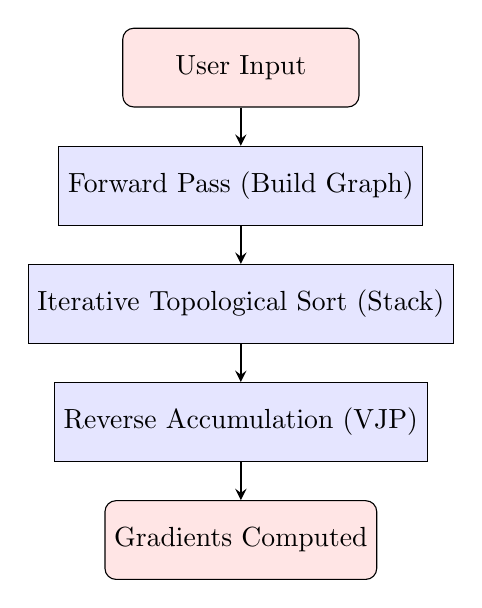
\begin{tikzpicture}[
    node distance=1.5cm,
    startstop/.style={rectangle, rounded corners, minimum width=3cm, minimum height=1cm,text centered, draw=black, fill=red!10},
    process/.style={rectangle, minimum width=3cm, minimum height=1cm, text centered, draw=black, fill=blue!10},
    arrow/.style={thick,->,>=stealth}
]

\node (start) [startstop] {User Input};
\node (forward) [process, below of=start] {Forward Pass (Build Graph)};
\node (topo) [process, below of=forward] {Iterative Topological Sort (Stack)};
\node (backward) [process, below of=topo] {Reverse Accumulation (VJP)};
\node (end) [startstop, below of=backward] {Gradients Computed};

\draw [arrow] (start) -- (forward);
\draw [arrow] (forward) -- (topo);
\draw [arrow] (topo) -- (backward);
\draw [arrow] (backward) -- (end);

\end{tikzpicture}
\caption{Execution pipeline of the MiniAD reverse-mode automatic differentiation engine.}
\label{fig:ad_flowchart}
\end{figure}

\subsection{Phase 1: Dynamic Graph Construction}

During forward execution, each overloaded operator constructs a new \texttt{Tensor} node. The node stores:

\begin{itemize}
    \item The computed numerical result in \texttt{data}
    \item References to differentiable parents in \texttt{\_prev}
    \item A closure implementing the local VJP in \texttt{\_backward}
\end{itemize}

Because parent references are recorded only when \texttt{requires\_grad=true}, non-differentiable branches are structurally pruned from the graph. The computational graph therefore emerges implicitly from standard Julia expressions, without requiring a separate graph-building interface.

\subsection{Phase 2: Iterative Topological Scheduling}

To ensure correct gradient propagation, a node must be processed only after all downstream consumers have contributed to its gradient. This is achieved through a post-order traversal implemented via an explicit stack.

The full implementation of the iterative topological sort is provided in Appendix~\ref{app:topo_sort}.

The traversal builds a post-order list \texttt{topo}. Reversing this list yields a valid reverse-topological order, ensuring that when \texttt{node.\_backward()} is executed, \texttt{node.grad} already equals the total derivative accumulated from all downstream paths.

\subsection{Reverse Replay Invariant}

The correctness of reverse-mode AD relies on the following invariant:

\begin{quote}
When a node's pullback is executed, its gradient field already stores the complete $\partial L/\partial(\texttt{node})$ accumulated from all consumers.
\end{quote}

This invariant is guaranteed by the post-order construction followed by reverse iteration. The output node is first seeded with $\partial L/\partial L = 1$, and successive pullbacks propagate sensitivities backward via in-place accumulation.

\subsection{Stability Considerations}

The stack-based implementation avoids recursion depth limits and supports arbitrarily deep computational graphs. Combined with structural pruning at the node level, this yields a memory-stable and execution-safe reverse-mode engine suitable for both neural networks and differentiable physical models.

\section{Broadcast-Based Elementwise Differentiation}

MiniAD integrates with Julia's broadcasting mechanism to support elementwise operations efficiently. Instead of hard-coding primitives, we use a custom \texttt{BroadcastStyle} and a backward rule registry. This allows operations like \texttt{sin.(x)} or \texttt{x .+ y} to automatically participate in the AD graph. Detailed implementation of the broadcast registry, custom style, and shape-correct gradient reduction (\texttt{unbroadcast}) is detailed in Appendix~\ref{app:broadcast}.


\section{Integrated Gradients for Interpretability}

While reverse-mode AD provides local sensitivity information, raw gradients often fail to capture feature importance in nonlinear models due to gradient saturation. To obtain a more faithful attribution measure, we implement \emph{Integrated Gradients} (IG), which computes feature attributions by integrating gradients along a straight-line path from a baseline input $x_0$ to the target input $x$.

For a scalar-valued model $F$, the $i$-th attribution is defined as:
\begin{equation}
\mathrm{IG}_i(x) 
= (x_i - x_{0,i}) 
\int_{0}^{1}
\frac{\partial F\big(x_0 + \alpha(x-x_0)\big)}{\partial x_i}
\, d\alpha.
\end{equation}

In practice, this integral is approximated using a Riemann sum with $m$ steps:
\begin{equation}
\mathrm{IG}(x) 
\approx 
(x - x_0) \odot 
\frac{1}{m}
\sum_{k=1}^{m}
\nabla_x F\!\left(x_0 + \frac{k}{m}(x-x_0)\right),
\end{equation}
where $\odot$ denotes elementwise multiplication.

Our implementation supports both AD-based gradients and finite differences, ensuring applicability to both differentiable tensors and black-box functions. The full code listing and design details (such as 2D alignment and gradient resetting) are discussed in Appendix~\ref{app:ig_details}.

\subsection{Interpretability Across Domains}

Because the IG implementation operates purely on gradients, it can be applied uniformly to:
\begin{itemize}
    \item Neural networks built from MiniAD layers
    \item Differentiable physical models expressed using Tensor operations
    \item Scalar black-box functions via finite differences
\end{itemize}

This unifies sensitivity analysis across machine learning and physics-based simulations within a single computational framework.



\section{Numerical Experiments and Case Studies}
We demonstrate the efficacy of our from-scratch AD and IG implementation through two case studies: optimizing a physics-based projectile model and interpreting a neural network classifier.
These experiments validate that the engine correctly handles gradient propagation for both explicit physical equations and learned black-box functions.

\subsection{Case Study I: Physics-Based Model --- Robotic Projectile Motion}
This case study utilizes the AD engine in two distinct ways: first for parameter optimization (Gradient Descent), and second for model interpretability (Integrated Gradients).

\subsubsection{Optimization of Trajectory}
The goal is to optimize the launch velocity $v$ and angle $\theta$ of a projectile to hit a target hoop at coordinates $(4.0, 3.1)$. The loss function is defined as the squared Euclidean distance between the projectile's position at the target x-coordinate and the hoop's height:
\[ L(v, \theta) = (y_{\text{pred}}(v, \theta) - h_{\text{hoop}})^2 \]
Using our AD engine, we compute $\nabla L$ and perform gradient descent. Figure~\ref{fig:netball_traj} shows the optimization progress from an initial failing trajectory to a successful shot.

\begin{figure}[H]
    \centering
    \includegraphics[width=0.8\textwidth]{netball_optimized_en.png}
    \caption{Trajectory optimization using reverse-mode AD. The red line shows the optimized path hitting the target hoop.}
    \label{fig:netball_traj}
\end{figure}

\subsubsection{Explainability with IG}
We apply Integrated Gradients to understand the sensitivity of the final trajectory height with respect to the launch parameters. Figure~\ref{fig:netball_ig} illustrates the attribution scores, indicating which parameter (velocity or angle) had a more significant impact on the final outcome relative to the baseline.

\begin{figure}[H]
    \centering
    \includegraphics[width=0.6\textwidth]{netball_ig.png}
    \caption{Integrated Gradients attribution for the Netball model, showing the contribution of velocity and angle to the result.}
    \label{fig:netball_ig}
\end{figure}

\subsection{Case Study II: Neural Model --- Feature Importance in Iris Classification}
We train a Multi-Layer Perceptron (MLP) on the Iris dataset~\cite{fisher1936use} to demonstrate the engine's capability in a standard deep learning context. The network consists of input, hidden, and output layers with ReLU activations, trained using Cross-Entropy loss.

\subsubsection{Training Performance}
The model is trained for 100 epochs using SGD. The loss curve in Figure~\ref{fig:iris_loss} confirms the correct implementation of the backward pass through the composition of linear and non-linear layers.

\begin{figure}[H]
    \centering
    \includegraphics[width=0.6\textwidth]{iris_loss.png}
    \caption{Training loss for the MLP on the Iris dataset, validating the AD engine's stability.}
    \label{fig:iris_loss}
\end{figure}

\subsubsection{Feature Attribution}
Using IG, we analyze the importance of the four input features (Sepal/Petal Length/Width) for a specific prediction (e.g., Setosa). Figure~\ref{fig:iris_ig} highlights the most influential features driving the model's decision, providing transparency to the "black box" neural network.

\begin{figure}[H]
    \centering
    \includegraphics[width=0.6\textwidth]{iris_ig.png}
    \caption{Feature importance attribution for an Iris Setosa prediction.}
    \label{fig:iris_ig}
\end{figure}

\section{Conclusion}
This work presented a minimalist yet functional implementation of Reverse-Mode Automatic Differentiation and Integrated Gradients in Julia. By decomposing programs into computational graphs of primitive operations, we demonstrated how exact gradients can be computed efficiently. The application of this engine to both a physics-based optimization problem and a neural network classification task highlights the universality of the approach. The project serves as a pedagogical bridge between the theoretical foundations of differentiable programming and its practical application in model interpretability.

\begin{thebibliography}{9}
\bibitem{griewank2008evaluating}
Griewank, A., \& Walther, A. (2008). Evaluating derivatives: principles and techniques of algorithmic differentiation. SIAM.

\bibitem{sundararajan2017axiomatic}
Sundararajan, M., Taly, A., \& Yan, Q. (2017). Axiomatic attribution for deep networks. In International Conference on Machine Learning (pp. 3319-3328). PMLR.

\bibitem{baydin2017automatic}
Baydin, A. G., Pearlmutter, B. A., Radul, A. A., \& Siskind, J. M. (2017). Automatic differentiation in machine learning: a survey. Journal of Machine Learning Research, 18(153), 1-43.

\bibitem{bezanson2017julia}
Bezanson, J., Edelman, A., Karpinski, S., \& Shah, V. B. (2017). Julia: A fresh approach to numerical computing. SIAM review, 59(1), 65-98.

\bibitem{fisher1936use}
Fisher, R. A. (1936). The use of multiple measurements in taxonomic problems. Annals of eugenics, 7(2), 179-188.

\bibitem{paszke2019pytorch}
Paszke, A., Gross, S., Massa, F., Lerer, A., Bradbury, J., Chanan, G., ... \& Chintala, S. (2019). PyTorch: An imperative style, high-performance deep learning library. In Advances in neural information processing systems (pp. 8026-8037).
\end{thebibliography}



\appendix
\section{Appendix}
\subsection{Algorithms} \label{app:algorithms}
\begin{algorithm}[H]
\caption{Reverse-Mode AD via Iterative Topological Sort}
\label{alg:reverse-ad}
\begin{algorithmic}[1]
\Require Output node $y$ (scalar \texttt{Tensor})
\Ensure Gradients stored in \texttt{grad} fields of all reachable nodes
\State \textbf{Phase 1: Iterative Topological Sort}
\State $\texttt{topo} \leftarrow \text{Empty List}$
\State $\texttt{visited} \leftarrow \text{Empty Set}$
\State $\texttt{stack} \leftarrow [(y, \textbf{false})]$ \Comment{Tuple: (node, processed\_flag)}
\While{$\texttt{stack}$ is not empty}
    \State $(v, \text{processed}) \leftarrow \textsc{Pop}(\texttt{stack})$
    \If{$v \notin \texttt{visited}$}
        \If{\text{processed}}
            \State $\textsc{Push}(\texttt{visited}, v)$
            \State $\textsc{Push}(\texttt{topo}, v)$ \Comment{Post-order insertion}
        \Else
            \State $\textsc{Push}(\texttt{stack}, (v, \textbf{true}))$
            \ForAll{$parent \in v.\_prev$}
                 \If{$parent \notin \texttt{visited}$}
                    \State $\textsc{Push}(\texttt{stack}, (parent, \textbf{false}))$
                 \EndIf
            \EndFor
        \EndIf
    \EndIf
\EndWhile
\State \textbf{Phase 2: Reverse Accumulation}
\State $y.\texttt{grad} \leftarrow 1$
\ForAll{$v \in \textsc{Reverse}(\texttt{topo})$}
  \State $v.\texttt{\_backward}()$ \Comment{Executes VJP closure}
\EndFor
\end{algorithmic}
\end{algorithm}

\begin{algorithm}[H]
\caption{Integrated Gradients using Reverse-Mode AD}
\label{alg:ig-ad}
\begin{algorithmic}[1]
\Require Model $F(\cdot)$, input $x$, baseline $x'$, steps $m$, optional target index
\Ensure Attribution vector $\mathrm{IG}(x)$
\State $\Delta \leftarrow x-x'$, \quad $G \leftarrow 0$
\For{$k=1$ to $m$}
  \State $\alpha \leftarrow k/m$
  \State $z \leftarrow x' + \alpha \Delta$
  \State Wrap $z$ as input \texttt{Tensor} and compute scalar output $y$
  \State \textsc{Backward}$(y)$ to obtain $\nabla_x F(z)$
  \State $G \leftarrow G + \nabla_x F(z)$
\EndFor
\State $\bar{G} \leftarrow G/m$
\State $\mathrm{IG}(x) \leftarrow \Delta \odot \bar{G}$
\end{algorithmic}
\end{algorithm}

\subsection{Implementation of Iterative Topological Sort} \label{app:topo_sort}
The iterative topological sort ensures stack-safety for deep graphs.
\begin{lstlisting}[language=Julia, caption={Iterative topological traversal and reverse replay}]
function backward_iterative(root::Tensor; init_grad=nothing)
    if !root.requires_grad
        return nothing
    end

    topo = Tensor[]
    visited = Set{Tensor}()
    stack = [(root, false)]

    while !isempty(stack)
        curr, processed = pop!(stack)
        if curr in visited
            continue
        end

        if processed
            push!(visited, curr)
            push!(topo, curr)
        else
            push!(stack, (curr, true))
            for parent in curr._prev
                if parent ∉ visited
                    push!(stack, (parent, false))
                end
            end
        end
    end

    root.grad .= (init_grad === nothing ? 1.0 : init_grad)

    for node in reverse(topo)
        node._backward()
    end
end
\end{lstlisting}

\subsection{Implementation of Broadcast Differentiation} \label{app:broadcast}
While matrix multiplication and reduction operators are implemented explicitly, most elementwise operations in MiniAD are handled through Julia's broadcasting mechanism. Instead of defining separate forward and backward logic for each primitive (e.g., addition, multiplication, trigonometric functions), we integrate directly with Julia's broadcast infrastructure and implement a modular backward rule registry.

\subsubsection{Custom Broadcast Style}

MiniAD defines a custom \texttt{TensorStyle} to intercept broadcasted operations:

\begin{lstlisting}[language=Julia, caption={Custom broadcast style definition}]
struct TensorStyle <: BroadcastStyle end
Base.BroadcastStyle(::Type{Tensor}) = TensorStyle()
Base.BroadcastStyle(::TensorStyle, ::BroadcastStyle) = TensorStyle()
Base.BroadcastStyle(::BroadcastStyle, ::TensorStyle) = TensorStyle()

broadcastable(t::Tensor) = t
\end{lstlisting}

This allows expressions such as \texttt{a .+ b}, \texttt{sin.(x)}, or \texttt{exp.(x)} to construct differentiable graph nodes automatically.

\subsubsection{Backward Rule Registry}

Rather than embedding gradient logic inside the broadcast dispatcher, we maintain a registry mapping primitive functions to their backward rules:

\begin{lstlisting}[language=Julia, caption={Broadcast backward rule registry}]
const BROADCAST_RULES = IdDict{Any,Function}()

function register_broadcast_rule!(f, rule::Function)
    BROADCAST_RULES[f] = rule
end
\end{lstlisting}

When a broadcasted operation is executed, MiniAD:

\begin{enumerate}
    \item Extracts raw data from \texttt{Tensor} arguments
    \item Performs the forward broadcast computation
    \item Constructs a new \texttt{Tensor} node
    \item Looks up the corresponding backward rule from the registry
    \item Attaches the rule as the node's \texttt{\_backward} closure
\end{enumerate}

If no rule is registered, an explicit error is raised, preventing silent gradient failures.

\subsubsection{Shape-Correct Gradient Reduction: \texttt{unbroadcast}}

Broadcasted operations may expand singleton dimensions. During backpropagation, gradients must therefore be reduced back to the original operand shape. This is handled by the \texttt{unbroadcast} operator:

\begin{lstlisting}[language=Julia, caption={Gradient shape reduction for broadcasted ops}]
function unbroadcast(out_grad::AbstractArray, orig_size::Tuple)
    g = out_grad

    while ndims(g) > length(orig_size)
        g = sum(g, dims=1)
    end

    for d in 1:length(orig_size)
        if orig_size[d] == 1 && size(g, d) != 1
            g = sum(g, dims=d)
        end
    end

    return reshape(g, orig_size)
end
\end{lstlisting}

This ensures that the gradient passed back to each operand matches its original dimensions, preserving consistency across scalar, vector, and matrix broadcasts.

\subsubsection{Example: Elementwise Multiplication}

For example, the broadcast rule for elementwise multiplication is registered as:

\begin{lstlisting}[language=Julia]
register_broadcast_rule!(*, (out, res, args...) -> begin
    x, y = args
    if x isa Tensor && x.requires_grad
        val_y = y isa Tensor ? y.data : y
        x.grad .+= unbroadcast(out.grad .* val_y, size(x.data))
    end
    if y isa Tensor && y.requires_grad
        val_x = x isa Tensor ? x.data : x
        y.grad .+= unbroadcast(out.grad .* val_x, size(y.data))
    end
end)
\end{lstlisting}

The backward rule directly implements the local derivative
\[
\frac{\partial (x \cdot y)}{\partial x} = y, \quad
\frac{\partial (x \cdot y)}{\partial y} = x,
\]
while ensuring correct dimensional reduction.

\subsubsection{Extensibility}

This registry-based design cleanly separates forward semantics from backward logic. New differentiable primitives can be added without modifying the core AD engine—only a corresponding broadcast rule needs to be registered.

Compared to monolithic AD implementations, this approach provides a modular and extensible differentiation framework while remaining minimal in code complexity.

\subsection{Details of Integrated Gradients} \label{app:ig_details}
\subsubsection{Implementation in MiniAD}

The implementation follows the definition directly:

\begin{lstlisting}[language=Julia, caption={Integrated Gradients implementation in MiniAD}]
function integrated_gradients(model, input, baseline;
    steps::Int=50, target=nothing, method=:ad)

    x = _align2d(input)
    x0 = _align2d(baseline)

    diff = x .- x0
    total_grads = zeros(size(x))

    for s in 1:steps
        α = s / steps
        z = x0 .+ α .* diff

        if method == :ad
            xt = Tensor(z, _op="Input")
            out = model(xt)
            y = to_scalar(out; target=target)

            if model isa Chain
                zero_grad!(model)
            end

            xt.grad .= 0.0
            y.grad .= 0.0

            backward(y)
            total_grads .+= xt.grad

        elseif method == :fd
            g, _ = grad_fd(model, copy(z))
            total_grads .+= g
        end
    end

    avg_grads = total_grads ./ steps
    return diff .* avg_grads
end
\end{lstlisting}

\subsubsection{Key Design Aspects}

\paragraph{2D Alignment.}
Inputs and baselines are internally normalized to 2D arrays to maintain consistency with the Tensor abstraction. This avoids special-case handling for scalars and vectors.

\paragraph{Dual Gradient Modes.}
The implementation supports two gradient computation modes:
\begin{itemize}
    \item \texttt{:ad} --- Uses the reverse-mode AD engine.
    \item \texttt{:fd} --- Uses finite differences for scalar-valued black-box functions.
\end{itemize}
This allows attribution analysis even when the model is not constructed using MiniAD tensors.

\paragraph{Gradient Resetting.}
Before each backward pass, gradients of the input tensor (and model parameters, if applicable) are reset. This prevents cross-step contamination during the Riemann approximation.

\paragraph{Completeness Property.}
The implementation satisfies the Completeness Axiom:
\[
\sum_i \mathrm{IG}_i(x) \approx F(x) - F(x_0),
\]
up to numerical approximation error from discretization. This provides a consistency check for attribution correctness.

\subsection{Member Contributions}
\begin{itemize}
    \item \textbf{Cao Yuan}: Proposed the core idea and integrated the code.
    \item \textbf{Liu Fei}: Participated in the toy example development and case optimization.
    \item \textbf{Jin Xuan}: Implemented complex main operators, conducted case verification, and wrote the paper.
    \item \textbf{Gao Jiaxuan}: Responsible for operator and method optimization.
    \item \textbf{Nan Jinyao}: Responsible for application case development, code integration, and paper writing.
\end{itemize}

\end{document}